\documentclass{standalone}
\usepackage{tikz}
\usepackage[]{xcolor}
\usetikzlibrary{calc}
\usepackage{bbold}
\usepackage{physics}

\newcommand{\mcG}{\mathcal{G}}

\graphicspath{{../figs/}}


\usepackage{amsmath, amsthm, amssymb}
\colorlet{coscolor}{blue}

\newcommand{\red}{\color{red}}
\newcommand{\blue}{\color{blue}}
%Colors

\definecolor{max}{rgb}{1,0.54,0.1}
\definecolor{medium}{rgb}{1,0.8,0.6}
\definecolor{min}{rgb}{1,0.9,0.8}
\begin{document}
\pagestyle{empty}
\newcommand{\xlength}{7}% tamaño horizontal de todas las figs
\newcommand{\xo}{0.5}% pos inicial en x de fig (a)
\newcommand{\yo}{0}% pos inicial en y de fig (a)
\newcommand{\sepxfigs}{1.03}% separación horizontal de las figuras
\newcommand{\sepyfigs}{4.8}% separación vertical de las figuras
\newcommand{\scalefont}{1.3}% scaling de las letras (a), (b), ...
\newcommand{\xoa}{0.35}% pos inicial en x de (a)
\newcommand{\yoa}{0}% pos inicial en x de (a)
\begin{tikzpicture}
% {
%%  fila 1 {
\node[anchor=north west] at (\xo, \yo) {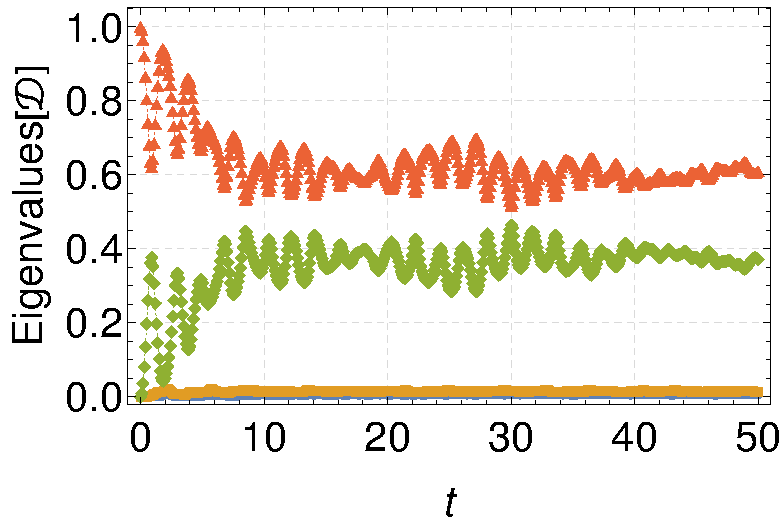
\includegraphics[width=\xlength cm]{choi_eigenvalues_regular1.pdf}};
\node[anchor=north west] at (\xo + \sepxfigs*\xlength, \yo)
{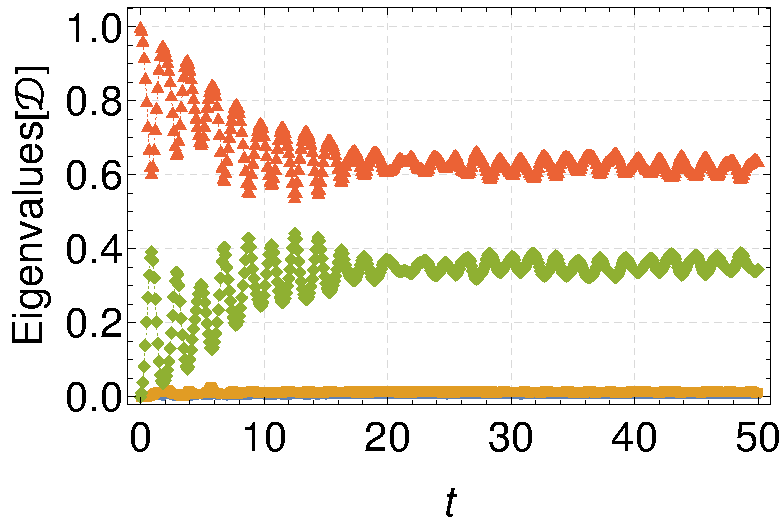
\includegraphics[width=\xlength cm]{choi_eigenvalues_regular2.pdf}};
\node[anchor=north west] at (\xo + 2*\sepxfigs*\xlength, \yo)
{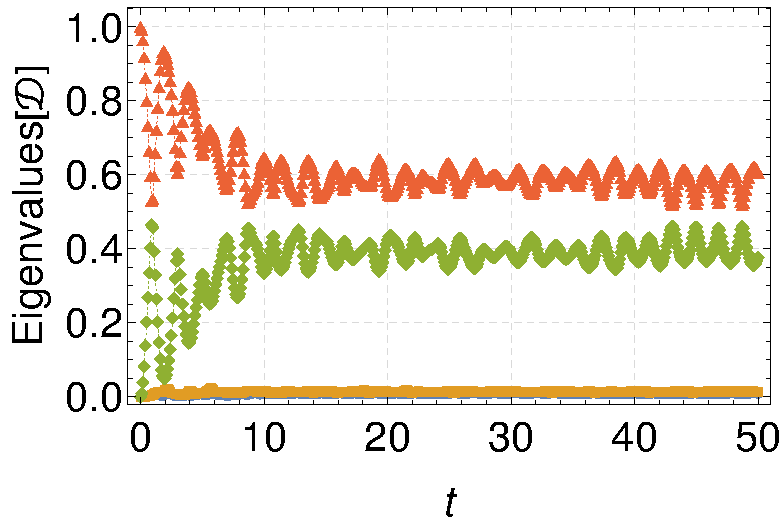
\includegraphics[width=\xlength cm]{choi_eigenvalues_regular3.pdf}};
%% }
%% fila 2 {
\node[anchor=north west] at (\xo, \yo - \sepyfigs) {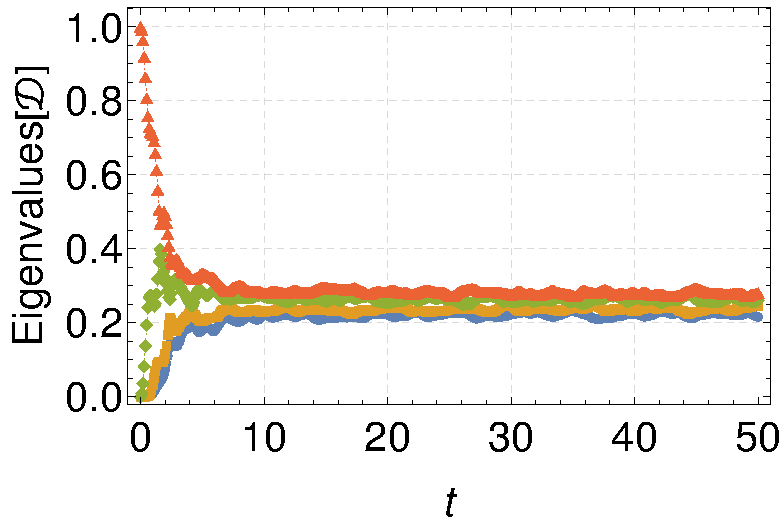
\includegraphics[width=\xlength cm]{choi_eigenvalues_chaotic1.pdf}};
\node[anchor=north west] at (\xo + \sepxfigs*\xlength, \yo - \sepyfigs)
{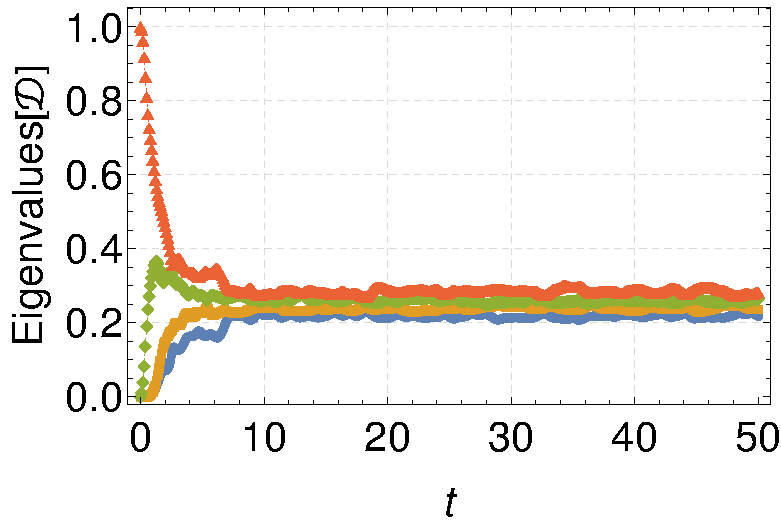
\includegraphics[width=\xlength cm]{choi_eigenvalues_chaotic2.pdf}};
\node[anchor=north west] at (\xo + 2*\sepxfigs*\xlength, \yo - \sepyfigs)
{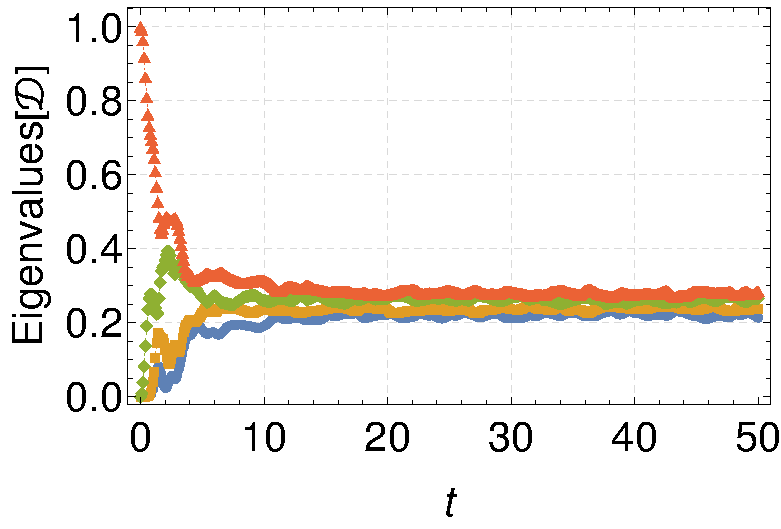
\includegraphics[width=\xlength cm]{choi_eigenvalues_chaotic3.pdf}};
%% }
%  } 
%
% letras {
\node[anchor=north west] at (\xoa, \yoa) {\scalebox{\scalefont}{(a)}};
\node[anchor=north west] at (\xoa + \sepxfigs*\xlength, \yoa) {\scalebox{\scalefont}{(b)}};
\node[anchor=north west] at (\xoa + 2*\sepxfigs*\xlength, \yoa) {\scalebox{\scalefont}{(c)}};
\node[anchor=north west] at (\xoa + 2*\sepxfigs*\xlength, \yoa) {\scalebox{\scalefont}{(c)}};
\node[anchor=north west] at (\xoa, \yoa - \sepyfigs) {\scalebox{\scalefont}{(d)}};
\node[anchor=north west] at (\xoa + \sepxfigs*\xlength, \yoa - \sepyfigs) {\scalebox{\scalefont}{(e)}};
\node[anchor=north west] at (\xoa + 2*\sepxfigs*\xlength, \yoa - \sepyfigs) {\scalebox{\scalefont}{(f)}};
% }
\end{tikzpicture}
\end{document}